\documentclass{mwart} 
\usepackage[polish]{babel} 
\usepackage[utf8]{inputenc} 
\usepackage{polski} 
\usepackage[T1]{fontenc} 
\usepackage{graphicx}

\usepackage[margin=1cm]{geometry}




\frenchspacing 

\usepackage{indentfirst} 
\title{\Huge{Sprawozdanie z laboratorium nr 6 i 7 \\
Różne implementacje tablicy asocjacyjnej }}
\author{Agnieszka Wiśniewska, nr albumu: 200466}

\begin{document}

\maketitle

\section{Wprowadzenie}
Tablica asocjacyjna jest jednym z abstrakcyjnych typów danych. Przechowuje ona pary - unikatowy klucz oraz wartość (poprzez podanie klucza można otrzymać dostęp do wartości z nim związanych).

Tablica asocjacyjna została zaimplementowana na trzy różne sposoby, a każdy z nich został poddany analizie czasowej.

\section{Implementacja nr 1 - tablica dynamiczna}
Jak widać na Rysunku \ref{faarray} algorytm zaimplementowany na tablicy dynamicznej ma logarytmiczną złożoność obliczeniową (jest to dobrze widoczne dzięki użyciu krzywej dopasowania logn). 
\begin{figure}[!htp]
\centering
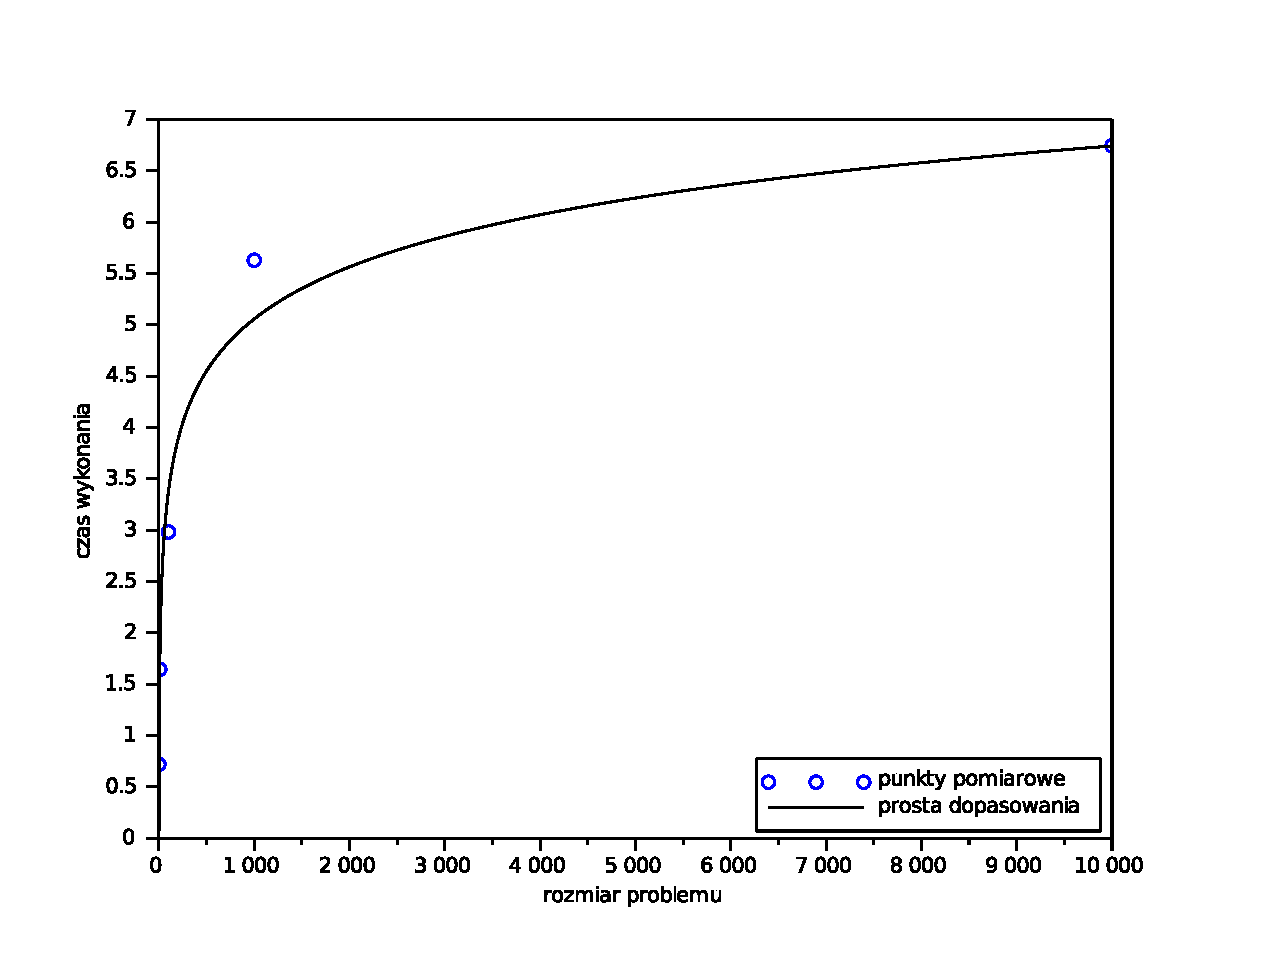
\includegraphics[width=\textwidth]{aarray.pdf}
\caption{Zależność czasu wykonywania algorytmu od rozmiaru problemu dla implementacji na tablicy dynamicznej. \label{faarray}} 
\end{figure}

\section{Implementacja nr 2 - tablica haszująca}
Na wykresie \ref{fhash} wyraźnie widać, że czas wykonania algorytmu przy tablicy haszującej jest w przybliżeniu stały (występują niewielkie odchylenia).

\begin{figure}[!htp]
\centering
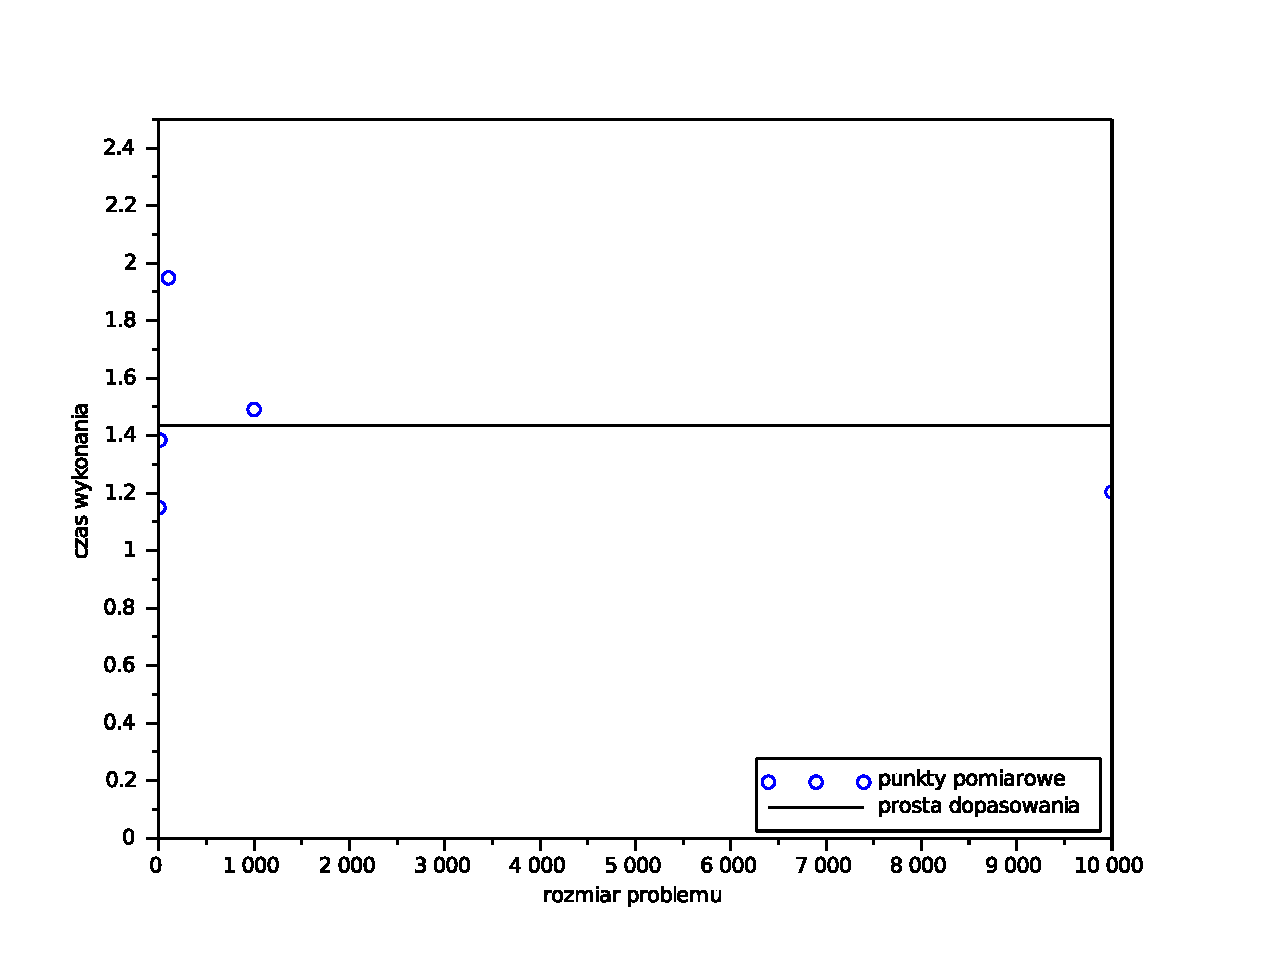
\includegraphics[width=\textwidth]{hash.pdf}
\caption{Zależność czasu wykonywania algorytmu od rozmiaru problemu dla tablicy haszującej. \label{fhash}} 
\end{figure}

\section{Implementacja nr 3 - drzewo binarne}
W przypadku wykresu nr \ref{ftree} złożoność jest taka, jak w przypadku tablicy dynamicznej - logarytmiczna (tutaj również użyto krzywej logn).

\begin{figure}[!htp]
\centering
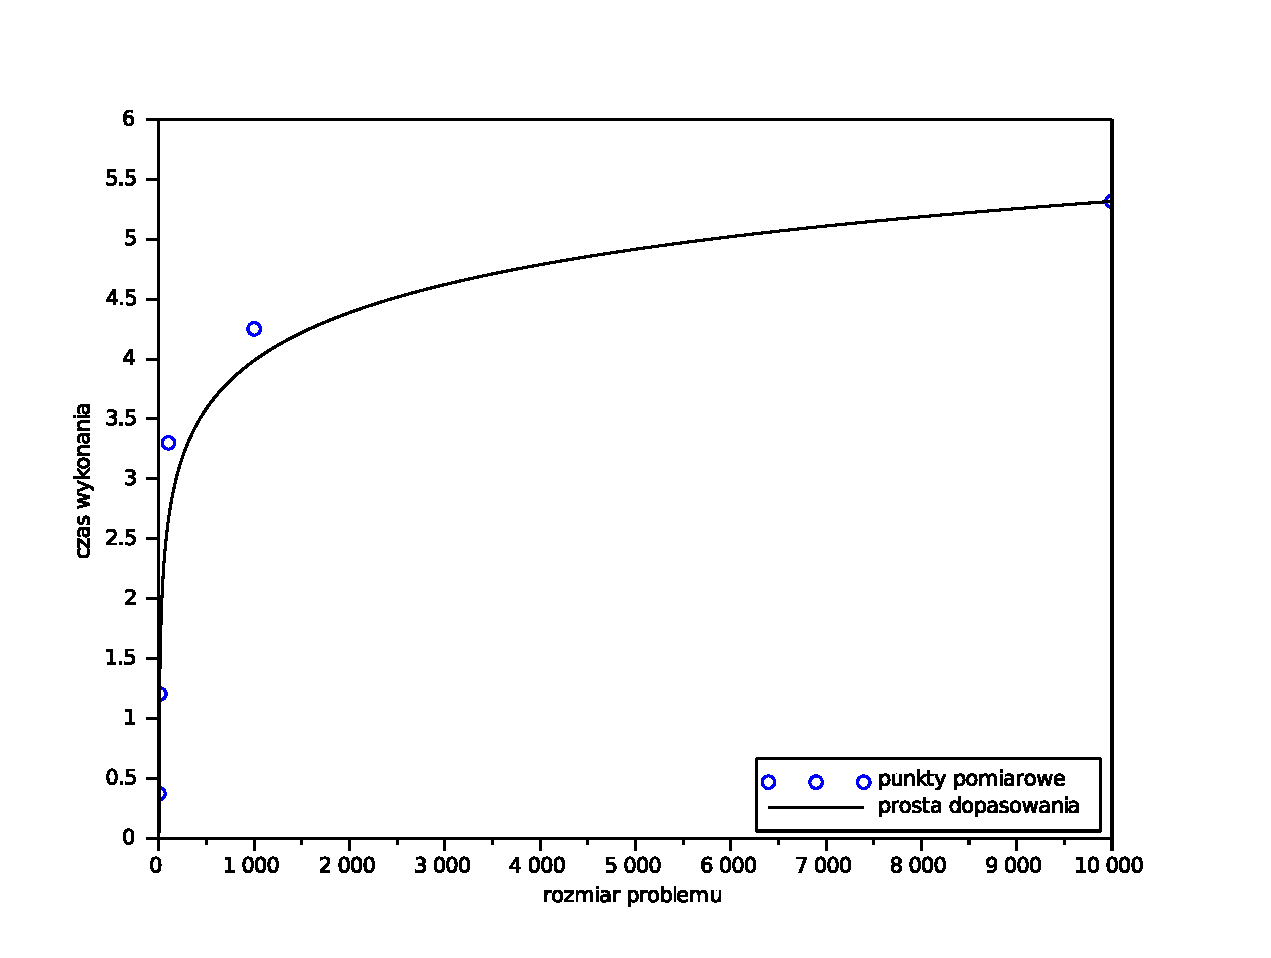
\includegraphics[width=\textwidth]{tree.pdf}
\caption{Zależność czasu wykonywania algorytmu od rozmiaru problemu dla drzewa binarnego. \label{ftree}} 
\end{figure}

\newpage
\section{Podsumowanie i wnioski}
\begin{itemize}
\item Udało się uzyskać rezultaty takie jak oczekiwano - w przybliżeniu stały czas wykonania algorytmu (niezależny od rozmiaru problemu) dla tablicy haszującej oraz złożoność logarytmiczną dla pozostałych dwóch przypadków.
\item Tablica asocjacyjna zaimplementowana na tablicy haszującej jest korzystnym rozwiązaniem dla dużych zestawów danych, zwłaszcza, gdy chcemy mieć dostęp do jej elementów w szybki sposób.
\end{itemize}




\end{document}